% !Mode:: "TeX:UTF-8"
\chapter{基于药物组合相似性网络的模型构建与求解}
\label{chap:theory}

\section{药物组合相似性假设及其验证}

\subsection{药物组合相似性计算}

本文使用药物分子指纹构建药物组合分子指纹,再使用药物组合分子指纹计算药物组合的相似系数。分子指纹是用于描述化合物结构的一种有效方法。该方法通过检测药物分子结构中的一些特定子结构是否存在,例如原子、键和环等,将分子结构转化为一系列0-1序列,从而对药物化合物的结构和性质进行编码和比较。这是一种快速、高效的结构描述工具,可用于计算化学、药物研究和分子设计等领域。由于药物分子指纹可以快速计算和比较,因此被广泛应用于虚拟筛选、化学信息学和计算化学等领域\supercite{21}。本文假设$d_i$表示药物$i$的分子指纹序列,$d_j$表示药物$j$的分子指纹序列:

\vspace{-1.5em}

\begin{equation*}
d_i = (d_{i1}, d_{i2}, \ldots, d_{in}),
\end{equation*}

\vspace{-1.5em}

\begin{equation*}
d_j = (d_{j1}, d_{j2}, \ldots, d_{in}),
\end{equation*}

\noindent 药物$d_i$和药物$d_j$横向拼接分子指纹序列获得药物组合$D$的分子指纹序列,即$D$表示为:

\vspace{-1.5em}

\begin{equation*}
\large D=(d_i, d_j) \text{ 或 } D=(d_j, d_i).
\end{equation*}

为了量化药物组合间的相似性,本文基于药物的分子指纹使用Tanimoto系数\supercite{23}计算药物组合的相似系数。Tanimoto系数是一种衡量两个分子之间相似程度的量化指标,当Tanimoto系数越高时,代表着两个分子的结构越相似。这种相似性可能意味着它们具有类似的生物活性、药理作用、代谢途径等。Tanimoto系数是一种广泛应用于化学结构相似性评估的指标,特别适用于评估分子之间的相似性。该系数的计算结果介于0和1之间,其中1表示两个分子完全相同,而0表示两个分子没有共同特征。根据该系数的定义,药物组合的Tanimoto系数矩阵如式(\ref{eq:dm}):

\vspace{-1em}

\begin{equation}
\mathbfit{T} = (T_{ij})_{m\times n},\label{eq:dm}
\end{equation}

\noindent 其中

\begin{equation}
T_{ij} = T(D_i, D_j) = \frac{|D_i \cap D_j|}{|D_i \cup D_j|},\label{eq:T}
\end{equation}

\noindent $m$为药物组合的个数,$D_i$和$D_j$分别为药物组合$i$和药物组合$j$。

在实际计算药物组合的Tanimoto系数时,需要考虑药物组合$D_i$和药物组合$D_j$之间的顺序以及它们自身分子指纹中单药横向拼接的顺序。这些顺序对计算结果都有影响,可能导致不同的结果。因此,在进行计算时,需要遍历四个不同的排列顺序,包括$D_i$和$D_j$之间的顺序以及它们自身分子指纹的顺序,然后选择最大值作为$D_i$和$D_j$之间的Tanimoto系数。通过这种方式,可以获得更准确、更可靠的结果。

\subsection{相似性假设的提出}

2015年,张乃千等人发现了“基因组信息相似的细胞系和分子结构相似的药物对应的药物反应谱更为相似”这一现象,构建了细胞系-药物双层网络模型,与局部线性方法相结合预测抗癌药物对于细胞系的敏感性,取得了较好的效果\supercite{15}。受此启发,本文拟通过药物组合-细胞系的协同得分构建DCSN模型。此时,在给定一个固定的细胞系的情况下,利用高相似药物组合的协同得分可以预测目标药物组合的协同得分。这种方式能够充分利用已有的相似药物组合信息,为预测目标药物组合的协同得分提供参考依据。DCSN模型的前提假设是“相似药物组合对固定细胞系具有相似的协同作用”。只有在该前提成立的情况下,模型才能有效进行预测,接下来本文将对该假设进行验证。

\subsection{相似性假设的验证}

\textbf{相似性阈值设置的可行性}

本文使用O'Neil数据集和NCI-ALMANAC数据集,分别计算了每个数据集药物组合之间的Tanimoto系数。由于Tanimoto系数矩阵数据量较大,因此本文采用了t-SNE降维方法(如式(\ref{eq:t1})、式(\ref{eq:t2})、式(\ref{eq:t3})),将数据降维到三维,以探索是否存在相似性关系\supercite{29}。t-SNE的核心思想是将高维空间中距离近的点映射到低维空间中距离仍然近的点,而将距离远的点映射到距离更远的点,以保留原始数据中的局部结构信息。通过最小化cost函数,t-SNE优化低维嵌入,使得低维空间中相似度与高维空间中相似度相近,从而实现数据降维与可视化。这一方法可以用于探索数据是否存在内在结构和规律。因此,本文采用了t-SNE方法,将高维的Tanimoto系数矩阵数据降维到三维,以便于观察和分析数据之间的相似性关系。

\begin{equation}
p_{ij} = \frac{\exp(-\lVert x_i - x_j \rVert^2 / 2\sigma^2)}{\sum_{k \neq l} \exp(-\lVert x_k - x_l \rVert^2 / 2\sigma^2)},\label{eq:t1}
\end{equation}

\begin{equation}
q_{ij} = \frac{(1 + \lVert y_i - y_j \rVert^2)^{-1}}{\sum_{k \neq l} (1 + \lVert y_k - y_l \rVert^2)^{-1}},\label{eq:t2}
\end{equation}

\begin{equation}
C = KL(P || Q) = \sum_i \sum_j p_{ij} \log \frac{p_{ij}}{q_{ij}}.\label{eq:t3}
\end{equation}

\noindent 其中,$p_{ij}$ 表示在高维空间中点 $x_i$ 与点 $x_j$ 的相似度,由高斯分布计算而得,分母为归一化系数;$q_{ij}$ 表示在低维空间中点 $y_i$ 与点 $y_j$ 的相似度,由t分布计算而得,分母为归一化系数;$KL$ 表示KL散度,用于度量两个概率分布之间的距离;$C$ 表示 cost 函数,用于评估低维空间与高维空间的相似度。

在t-SNE降维的实现过程中,需要注意Tanimoto系数矩阵是一个沿主对角线对称的矩阵,其中主对角线上的系数对应每种药物组合自身的相关系数全为1。因此,需要将矩阵的下三角元素赋值为0,并且只使用矩阵的上三角数据进行计算。t-SNE是基于相似度或距离矩阵进行降维的,只要相似度或距离矩阵保持不变,那么降维的结果也不会发生变化。将下三角数据设置为0相当于将这些数据作为距离矩阵的缺失值处理,不会对上三角数据的权重产生影响,从而不会对t-SNE的结果产生影响。具体而言,通过t-SNE将数据降至三维,并将其制作成三维散点图,如图\ref{fig:mts}和图\ref{fig:nts}所示。

\begin{figure}[H]
\centering
  \begin{minipage}{0.5\linewidth}
    \centering
    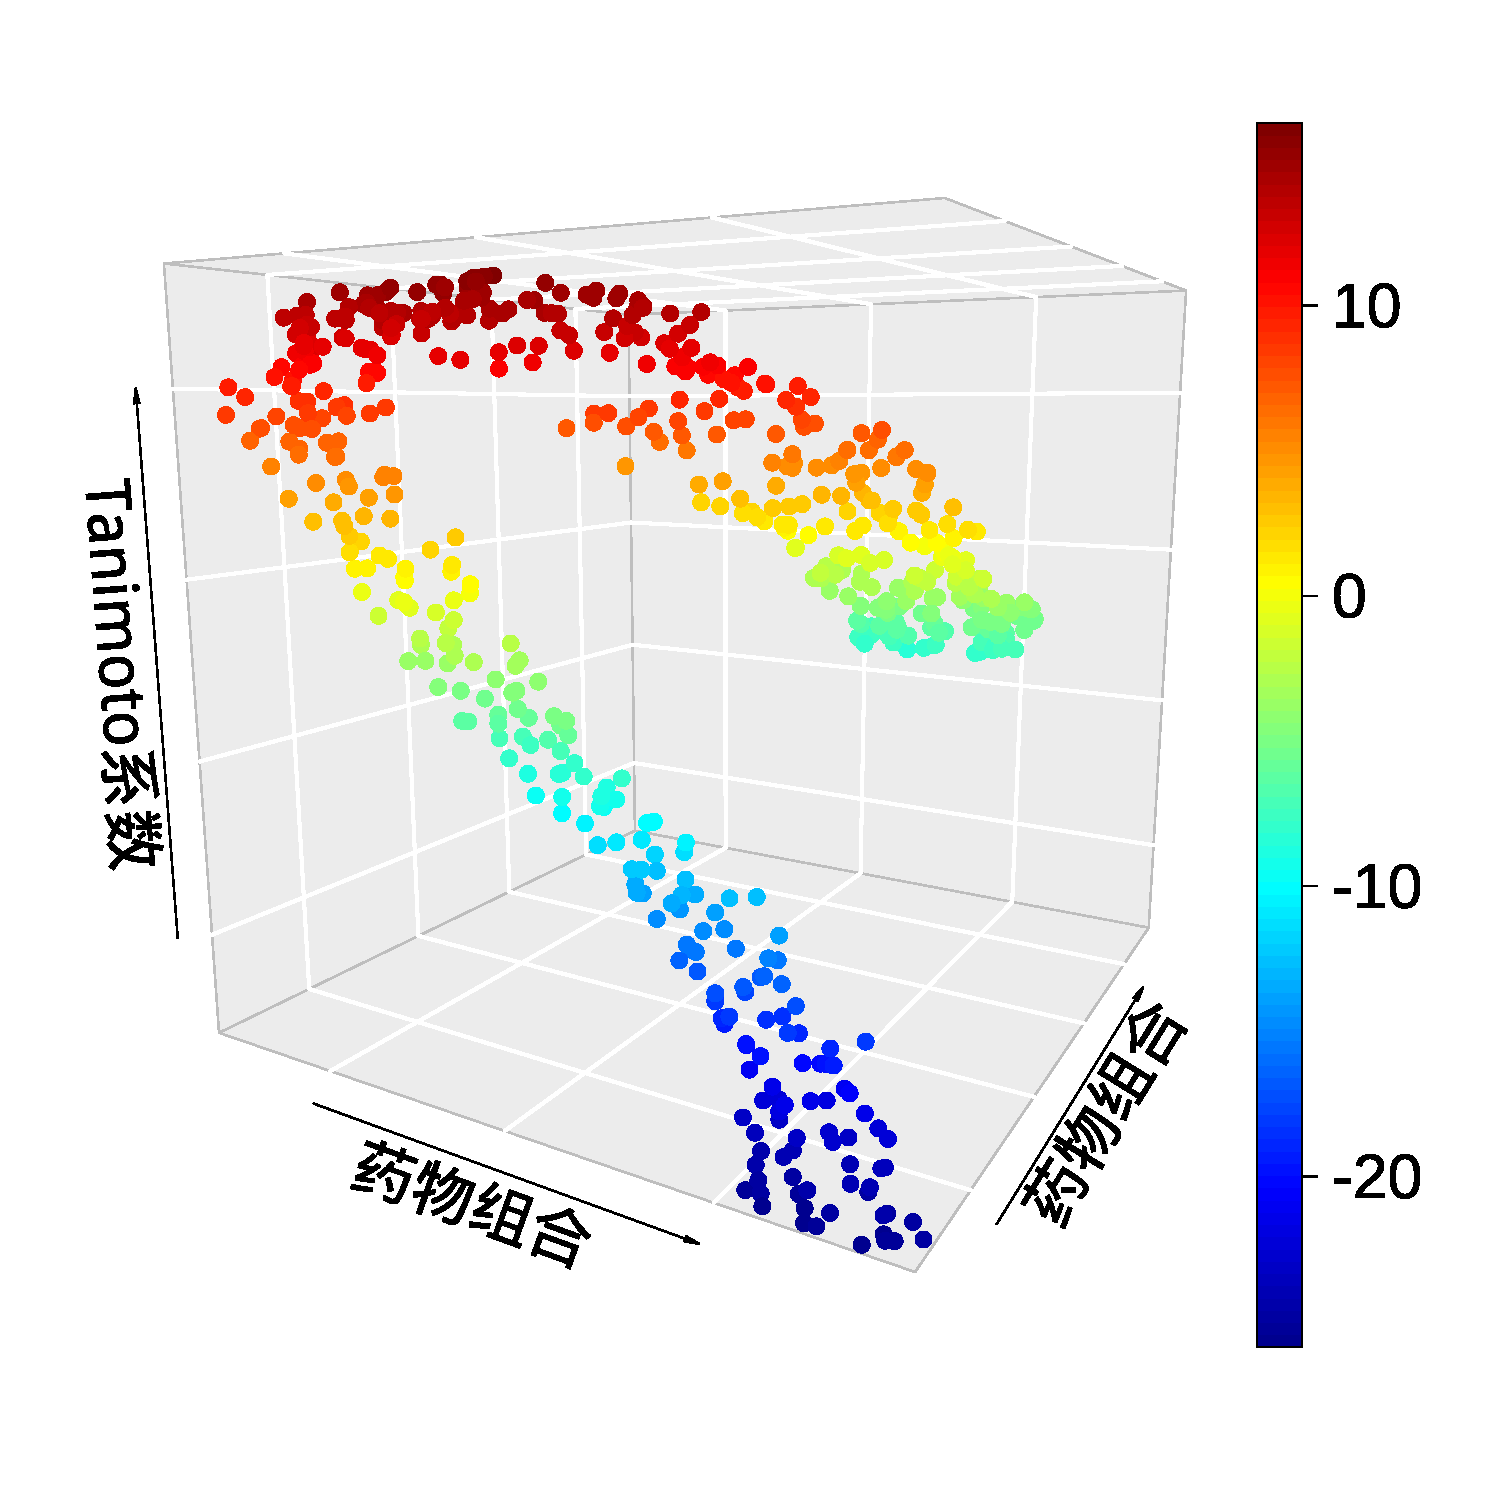
\includegraphics[width=\linewidth]{figures/o_t_sne.pdf}
    \caption{基于t-SNE的O'Neil数据集\\Tanimoto系数散点图}\label{fig:mts}
  \end{minipage}%
  \begin{minipage}{0.5\linewidth}
    \centering
    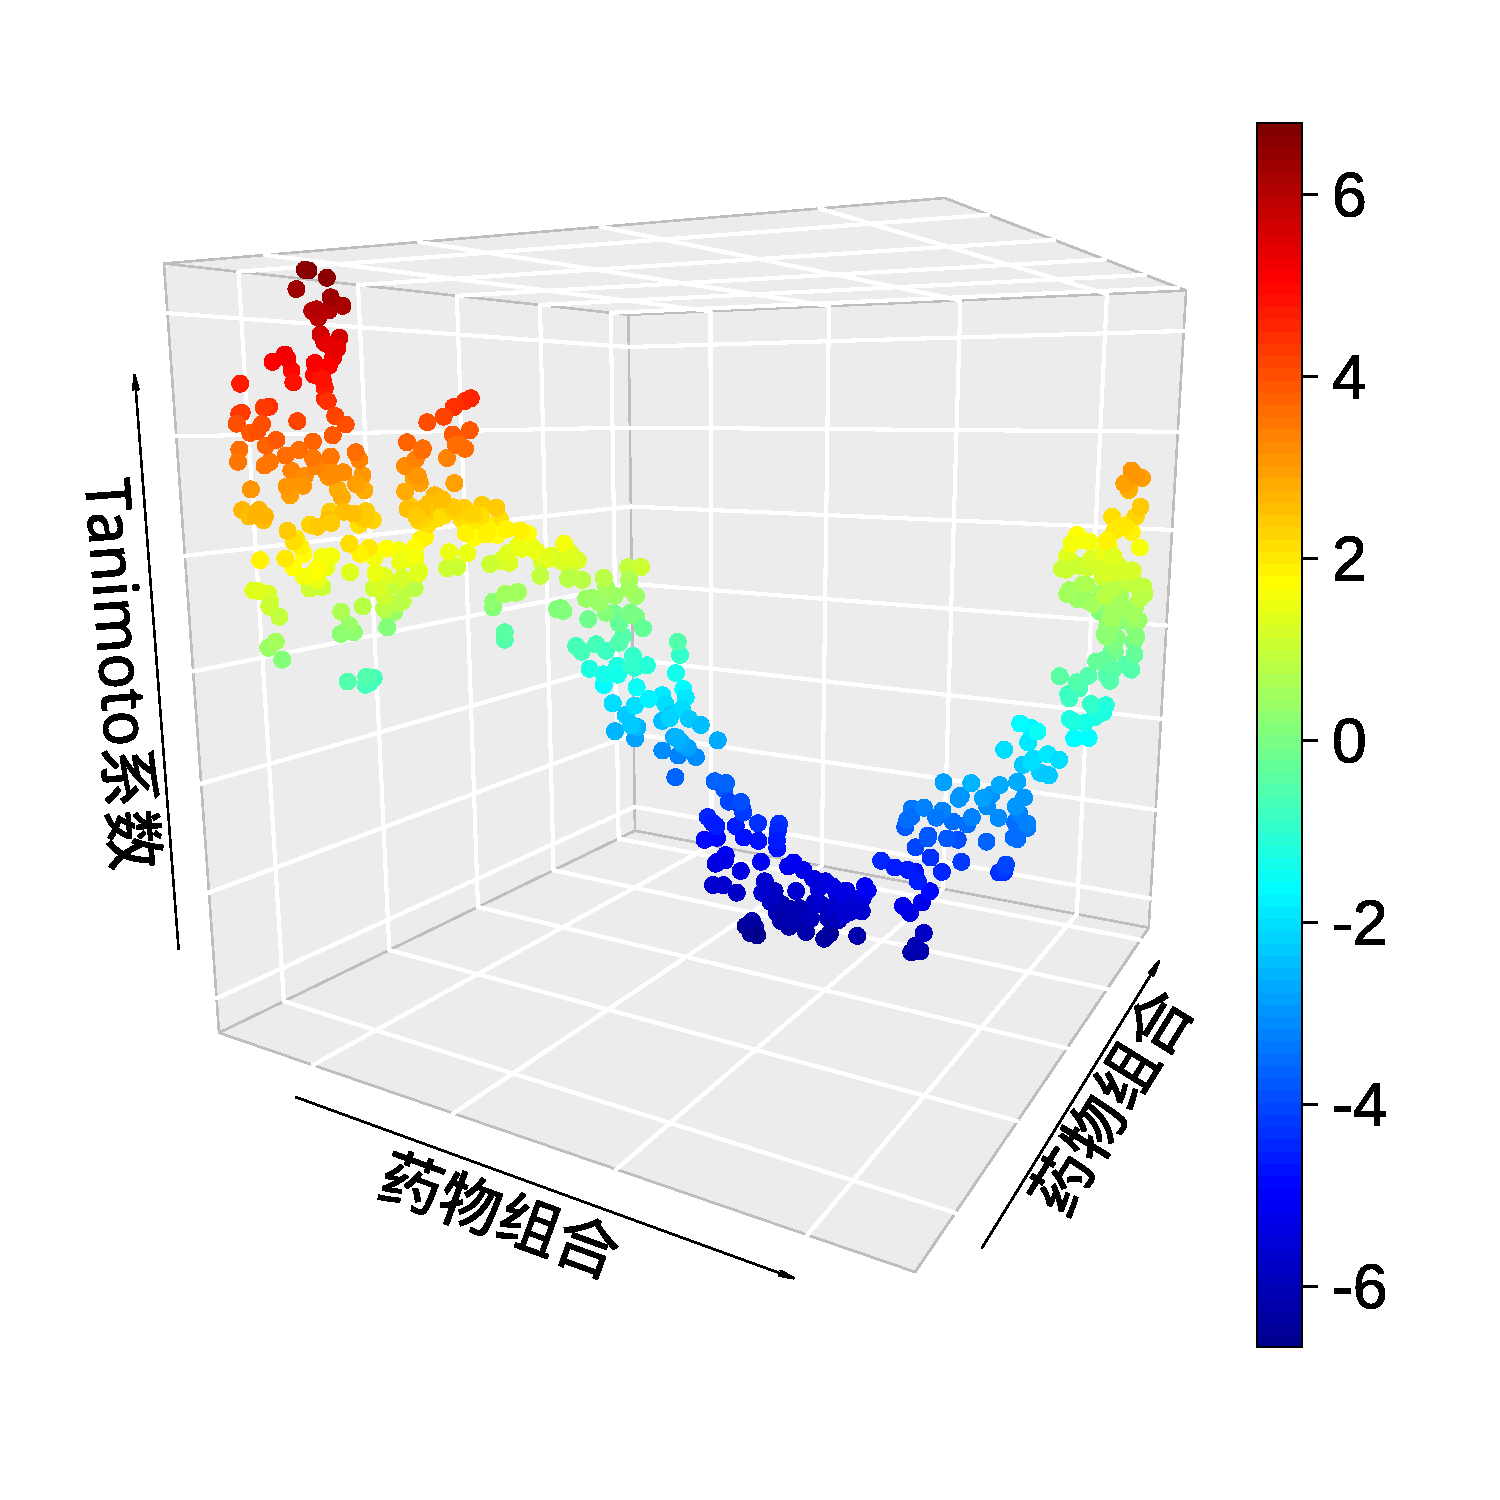
\includegraphics[width=\linewidth]{figures/n_t_sne.pdf}
    \caption{基于t-SNE的NCI-ALMANAC数据集\\Tanimoto系数散点图}\label{fig:nts}
  \end{minipage}
\end{figure}

观察三维散点图,无论使用哪个数据集,散点都呈现出一种类似于跨越整个三维空间的对角线簇的趋势。这暗示了数据集本身具有一定的内在结构,可以使用低维空间中的一条曲线簇来进行近似表示。这也表明,数据集中存在着某种相似性和规律性,这些特征可以通过降维后的曲线簇来进行表示。本文则认为,不同的数据点可能具有相似的特征或属性,因此它们在低维空间中会聚集成曲线簇。在高维空间中,数据点之间存在某种程度的相似性或相关性,而这种相似性或相关性在低维空间中被保留下来。同时,在低维空间中,数据点之间的距离关系也得到了保留。相距较远的点在三维空间中仍然相距较远,而相距较近的点在三维空间中也比较接近。这说明t-SNE算法可以在保留数据局部结构的同时,尽可能地减少不同类别之间的干扰。

\vspace{-1em}

\begin{equation}
\mathbfit{Hd} = \begin{bmatrix} T_1^{(1)} \\ \vdots \\ T_n^{(1)} \end{bmatrix}, \qquad 
\mathbfit{Ld} = \begin{bmatrix} T_1^{(2)} \\ \vdots \\ T_n^{(2)} \end{bmatrix}.
\label{eq:hdld}
\end{equation}

基于以上分析,本文认为可以利用Tanimoto系数并设置相似性系数的阈值来对数据集进行划分,以识别高相似性药物组合团和低相似性药物组合团。这种方法有助于进一步挖掘数据集中的相似性和规律性,以更好地理解数据集中的特征和属性。在前文提到的三维散点图中,可以通过在两个水平方向上进行横截面分割,将散点分成相应的高\texttt{\symbol{92}}低相似药物组合散点团。根据这些药物组合团的名称,可以将药物组合-细胞系的协同得分矩阵分成两个矩阵(\ref{eq:hdld})。具体而言,即根据式(\ref{eq:dm})和式(\ref{eq:T})计算的结果,药物组合可以分为两个团体,其中Tanimoto系数大于$α$的药物组合属于高相似药物组合团$\mathbfit{Hd}$,而Tanimoto系数小于$β$的药物组合则属于低相似药物组合团$\mathbfit{Ld}$。

\textbf{基于相似性阈值的协同得分分布}

假设药物组合个数为$m$,细胞系个数为$n$,药物组合$D_i$与细胞系$C_j$之间的协同得分表示为$S_{ij}$,药物组合-细胞系的协同得分矩阵表示为

\vspace{-1em}

\begin{equation}
\mathbfit{S} = (S_{ij})_{m\times n},
\end{equation}

\noindent 分别对$\mathbfit{Hd}$和$\mathbfit{Ld}$中对应的$S_i^{(1)}, S_i^{(2)}$进行Spearman相关系数的计算,如

% \vspace{-1em}

\begin{equation}
r_i^k=1-\frac{6\sum_{i=1}^n(S_i^{(k)}-S_i^{(k)})^2}{n(n^2-1)} \quad (k=1 \text{ 或 } k=2).
\label{eq:sp}
\end{equation}

这里在考察药物组合团的协同作用时,使用了Spearman相关系数\supercite{24}来度量最终高相似与低相似药物组合团的协同作用。Spearman相关系数可用于评估不同药物组合相似性和它们在协同作用方面的表现是否相似。具体而言,当两种药物组合的相似性越高时,如果它们在协同作用方面的表现也越相似,则它们的Spearman相关系数会更高;反之,当两种药物组合的相似性越低时,它们在协同作用方面的表现如果越不相似,则它们的Spearman相关系数会更低。高相似药物组合-细胞系协同得分的Spearman相关系数矩阵$\mathbfit{M_1}$和低相似药物组合-细胞系协同协同得分的Spearman相关系数矩阵$\mathbfit{M_2}$:

\vspace{-1em}

\begin{equation*}
\mathbfit{M_1} = \begin{pmatrix} r_1^{(1)} & r_2^{(1)} & \cdots & r_n^{(1)} \end{pmatrix}, 
\end{equation*}

\vspace{-1em}

\begin{equation*}
\mathbfit{M_2} = \begin{pmatrix} r_1^{(2)} & r_2^{(2)} & \cdots & r_n^{(2)} \end{pmatrix}.
\end{equation*}

基于O'Neil数据集的实验结果显示,当Tanimoto系数的临界值$α$被设定为0.60,临界值$β$被设定为0.52时,高低相似药物组合的数量近似相同,其中高相似性药物组合的数量为11个,低相似药物组合的数量为13个。针对这些数据,可以绘制两个药物组合团相关性分布的箱线图,如图\ref{fig:1g}所示。同时,基于NCI-ALMANAC数据集的实验结果显示,当Tanimoto系数的临界值$α$被设定为0.55,临界值$β$被设定为0.52时,高相似药物组合和低相似药物组合的数量近似相同。其中,高相似性药物组合的数量为38个,而低相似药物组合的数量为35个。根据这些数据,可以绘制两个药物组合团相关性分布的箱线图,如图\ref{fig:2g}所示。

\begin{figure}[H]
\centering
  \begin{minipage}{0.45\linewidth}
    \centering
    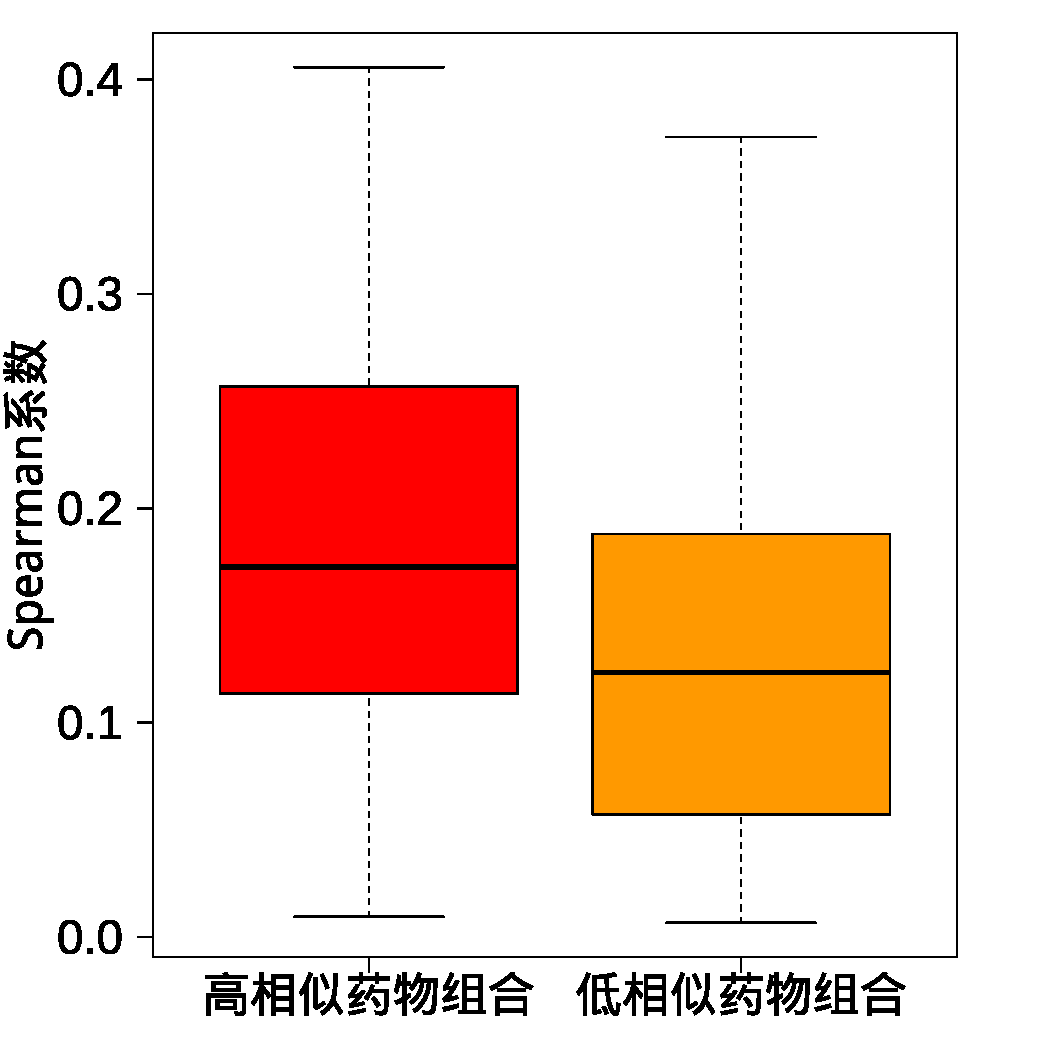
\includegraphics[width=\textwidth]{figures/O箱线图.pdf}
    \caption{O'Neil数据集\\药物组合相似性假设验证\label{fig:1g}}
  \end{minipage}%
  \begin{minipage}{0.45\linewidth}
    \centering
    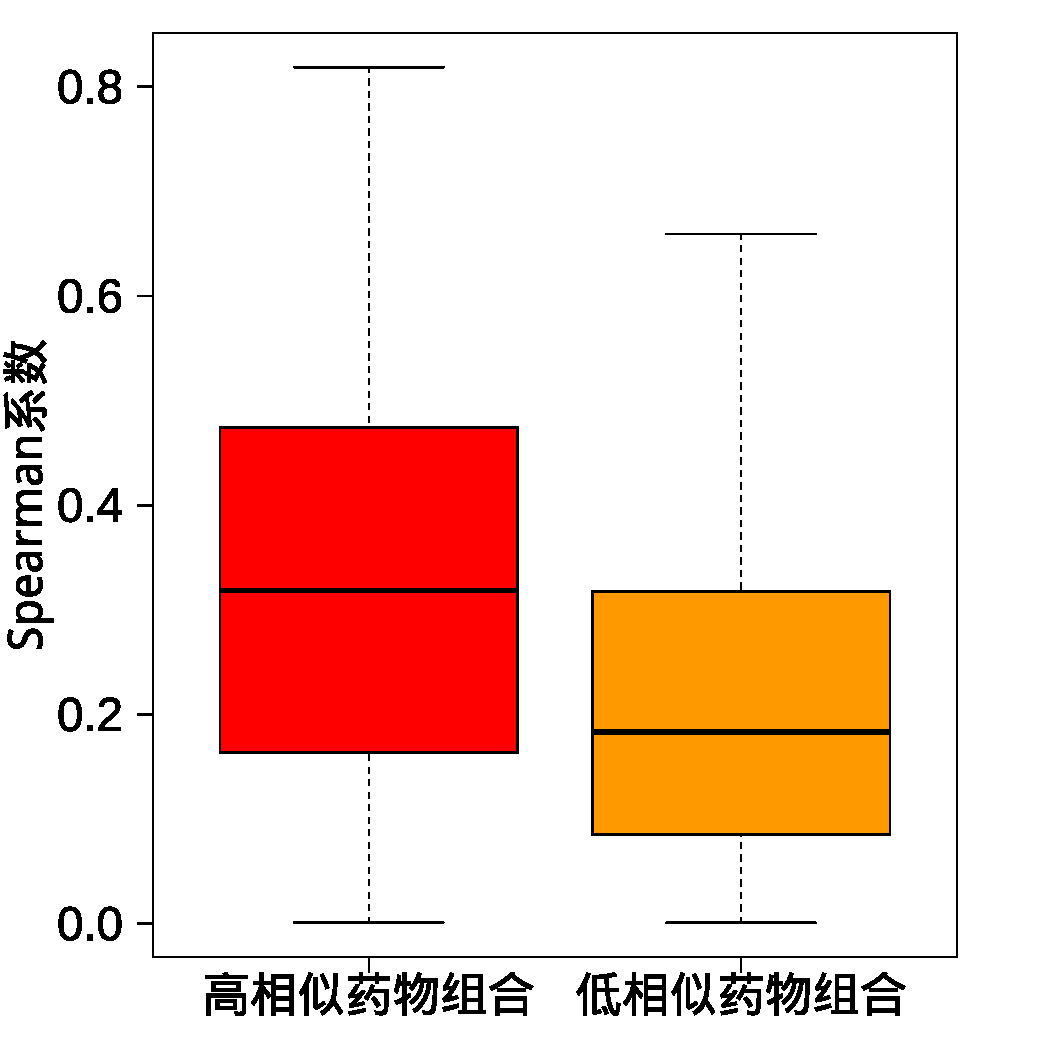
\includegraphics[width=\textwidth]{figures/NCI箱线图.pdf}
    \caption{NCI-ALMANAC数据集\\药物组合相似性假设验证\label{fig:2g}}
  \end{minipage}
\end{figure}

\vspace{-1em}

通过图\ref{fig:1g}和图\ref{fig:2g}可以更加清晰地了解高相似性药物组合和低相似药物组合之间的差异和共性。显然,高相似药物组合协同得分的Spearman相关系数明显高于低相似药物组合的Spearman相关系数,“相似药物组合对固定细胞系具有相似的协同作用”的假设验证成立,模型构建的前提条件成立。在此前提下,构建模型可以使用高相似药物组合去预测目标药物组合的协同作用。

\section{药物组合相似性网络模型的构建}

参考文献\cite{15}中基于药物相似性网络构建的单层网络预测模型中,认为与药物$D$化学结构相似性高的药物$D_j$与细胞系$C$的药物敏感性相比于其它药物与细胞系$C$的药物敏感性对模型的预测有更高的贡献。因此,该文献的模型给与药物$D$具有高相似的药物$D_j$对于细胞系$C$的药物敏感性以更高的权重,给与药物$D$具有低相似的药物对于细胞系$C$的药物敏感性以更低的权重,这里的权重函数$\omega(D,D_j)$是药物$D_j$与药物$D$的相关系数的单增函数,具体形式为:

\begin{equation}
\omega(D,D_j)=\exp\left(-\frac{[1-\rho(D,D_j)]^2}{2\tau^2}\right).\label{eq:znc}
\end{equation}

该权重函数$\omega(C,C_i)$基于高斯核函数$w(x_i, x_j)$扩展而来的。在许多ML方法中,经常需要定义一种权重函数来衡量不同样本之间的相似度或距离。高斯核函数是一种常用的权重函数,它以高斯(正态)分布的形式将权重分布在样本周围,其定义如下:

\vspace{-1em}

\begin{equation*}
w(x_i, x_j) = \exp\left(-\frac{{\|x_i - x_j\|^2}}{{2\sigma^2}}\right).
\end{equation*}

\noindent 其中,$w(x_i, x_j)$表示样本$x_i$和$x_j$之间的权重,$|x_i - x_j|$表示欧氏距离,$\sigma$表示高斯核函数的带宽(控制权重函数的宽窄程度)。在实际应用中,通常需要根据具体问题和数据的特点来选择适当的带宽参数$\sigma$。较小的$\sigma$会使得权重函数在样本周围的区域变得更加尖锐,更加注重局部相似性;而较大的$\sigma$会使得权重函数在整个样本空间内分布更均匀,更加注重全局相似性。

本文借鉴了药物敏感性预测的局部加权模型(\ref{eq:znc}),类似的提出了药物组合相似性网络模型(DCSN)的权重函数(\ref{eq:omg}):

\begin{equation}
\omega(D,D_j)=\exp\left(-\frac{[1-T(D,D_j)]^2}{2\tau^2}\right).
\label{eq:omg}
\end{equation}

\noindent 其中,$T(D,D_j)$表示药物组合$D$和$D_j$的Tanimoto系数,$τ$表示药物组合相似性降低时的衰减率。本文认为与药物组合$D$相似性高的药物组合对细胞系的协同作用相比于其它相似性低的药物组合对细胞系的协同作用对模型的预测有更高的贡献。因此,DCSN模型给与药物组合$D$具有高相似的药物组合以更高的权重,给与药物组合$D$具有低相似的药物组合以更低的权重。

DCSN模型构建如下:

\begin{equation}
\hat{S}_1(D,C) = \frac{\sum\limits_{i=1}^N \omega(D,D_j) \mathbfit{S}(D_j,C)}{\sum\limits_{i=1}^N \omega(D,D_j)}.
\end{equation}

\noindent 其中,$ω(D,D_j)$表示通过权重函数(\ref{eq:omg})计算药物组合$D_j$对于$D$的权重,$\mathbfit{S}(D_j,C)$表示药物组合$D_j$对于细胞系$C$的协同得分测试值,$\hat{S}_1(D,C)$表示药物组合$D$对于细胞系$C$的协同得分预测值。在实验过程中,发现归一化的加权网络模型效果比未归一化的模型效果更好,在使用邻居药物组合去预测目标药物组合的协同作用得分时,在加权和${\sum\limits_{i=1}^N \omega(D,D_j) \mathbfit{S}(D_j,C)}$后除以了权重和${\sum\limits_{i=1}^N \omega(D,D_j)}$,使得模型的预测效果更优。

\section{模型求解}

本文使用留一交叉验证\cite{25}训练模型,确定模型参数,使用Pearson相关系数(PCC)评估模型的预测性能,具体操作过程如下:从所有的协同得分数据中取出一个药物组合数据作为测试集,剩余数据作为训练集,在此训练集之上建立模型,再在测试集上进行预测;数据集中每一个药物组合的数据都被逐一取出作为测试集,并用剩余的数据作训练集,建立模型求解,于是得到所有药物组合协同得分的预测值。测试集的药物组合不包含在训练数据中,这可以用来评估模型的泛化能力。

在药物组合相似性网络模型中,需要确定两个超参数,分别是药物组合高相似的邻居数$N$和药物组合相似性降低时的衰减率$τ$。其中,药物组合高相似的邻居数$N$是基于药物组合相似性指标Tanimoto系数确定的。因此,该参数可以由另一个超参数——药物组合的相似性阈值平替来确定。该阈值限制了药物组合高相似的药物组合邻居的Tanimoto系数大小。

在实际实验的过程中,考虑使用PCC最大和均方误差(MSE)最小作为目标进行求解,但考虑到相关模型使用原始数据进行预测和评价,而DCSN模型使用标准化后的数据进行预测和评价,不同模型横向比较MSE不具备实际意义,所以最终选择使用PCC最大作为目标函数求解。PCC的取值范围在$-1$到$+1$之间,其中$-1$表示完全的负相关,$+1$表示完全的正相关,$0$表示无相关性。PCC的计算基于两个变量之间的协方差和各自的标准差:

\begin{equation*}
\text{PCC} = \frac{\sum_{i=1}^{n}(x_i - \bar{x})(y_i - \bar{y})}{\sqrt{\sum_{i=1}^{n}(x_i - \bar{x})^2}\sqrt{\sum_{i=1}^{n}(y_i - \bar{y})^2}}.
\end{equation*}

\noindent 其中,$n$ 是样本数量,$x_i$ 和 $y_i$ 是第 $i$ 个样本的两个变量的取值,$\bar{x}$ 和 $\bar{y}$ 分别是两个变量的均值。PCC 的取值范围在 $[-1, 1]$,当 PCC 的值接近 1 时,表示两个变量正相关;当 PCC 的值接近 -1 时,表示两个变量负相关;当 PCC 的值接近 0 时,表示两个变量无线性相关关系。

因此,根据超参数的种类,可以得到四种有不同求解区间的方法,分别使用不同的求解规则:

(1) 药物组合高相似的邻居数$N$指定范围为[2:200],药物组合相似性降低时的衰减率$τ$指定范围为[1:3],遍历所有可能的取值,以PCC最大为目标函数求解,基于该规则的求解方法称为\textbf{精细调参法}。

(2)	药物组合高相似的邻居数$N$指定范围为[2:100],药物组合相似性降低时的衰减率$τ$指定范围为[1:3],但各药物组合邻居数$N$取值统一,遍历所有可能的取值,以PCC最大为目标函数求解,基于该规则的求解方法称为\textbf{邻居数统一法}。

(3)	药物组合高相似的邻居数$N$指定范围为[2:100],各药物组合邻居数$N$取值统一,药物组合相似性降低时的衰减率$τ$指定范围为[1:3],各药物组合衰减率$τ$取值也统一,遍历所有可能的取值,以PCC最大为目标函数求解,基于该规则的求解方法称为\textbf{邻居数和衰减率统一法}。

(4)	药物组合高相似的邻居数$N$由药物组合相似性阈值限定,指定阈值可变范围为[0.5:1],取值间隔为0.001,药物组合相似性降低时的衰减率$τ$指定范围为[1:3],遍历所有可能的取值,以PCC最大为目标函数求解,基于该规则的求解方法称为\textbf{药物组合相似性阈值法}。

本文使用了这4种不同的方法对模型进行求解,每一种方法都得到了各自最优的超参数以及相应的评价指标。对于精细调参法而言,由于需要遍历两个可变参数,其计算量较大。相比之下,邻居数统一法在精细调参法的基础上,指定所有药物的一个可变参数统一取值,从而减小了计算量。邻居数和衰减率统一法在邻居数统一法的基础上,指定所有药物的可变参数都统一取值,进一步减少了计算量。而药物组合相似性阈值法则是在减少其中一个可变参数的计算量的基础上进行的,但仍需要遍历两个可变参数。在模型求解代码的实现过程中,本文为每一种方法的求解都采用了多进程并行计算,以充分利用CPU的算力资源,降低模型求解的时间成本。

\section{本章小结}

本章主要介绍了模型构建与求解的过程。首先,本文论证了药物组合的相似性可以通过计算药物分子指纹的Tanimoto系数来量化,同时需要考虑药物组合和单个药物分子指纹的排列顺序,并选择最大值作为药物组合的Tanimoto系数。其次,本文提出了前提假设,即“相似药物组合对固定细胞系具有相似的协同作用”。基于这一假设,采用t-SNE方法将数据降维到三维空间,发现数据点呈现出跨越整个三维空间的对角线簇趋势,所以可以通过设定相似性阈值划分高相似性药物组合团和低相似性药物组合团。同时,高相似性药物组合的协同得分的Spearman相关系数明显高于低相似性药物组合,验证了“相似药物组合对固定细胞系具有相似的协同作用”这一假设。最后,基于验证的结果,提出了DCSN模型。本章还给出了求解该模型超参数的4种不同方法和比较优势。